\subsection{Schritt 1 - Entwurf und Implementierung eines GP}

% TODO Eigenschaften LLT

\paragraph*{Entwurf eines Geschäftsprozesses}

Zur Untersuchung der Probleme soll ein Geschäftsprozess entworfen und als Saga-System implementiert werden. Der Durchlauf durch diesen Geschäftsprozess soll als LLT aufgefasst werden. Der Geschäftsprozess muss eine der in \ref{} beschriebenen Eigenschaften aufweisen, damit die Realisierung dieses Prozesses innerhalb einer Saga sinnvoll ist.  

Es besteht die Anforderung an den zu entwerfenden Prozess, dass dieser durch eine Menge von lokalen Transaktionen abbildbar sein muss. Außerdem muss es möglich sein, Kompensierungen für jede dieser Transaktionen zu formulieren. 

\paragraph*{Imaginärer Bestell- und Lieferprozess}

Als abzubildender Geschäftsprozess soll ein Bestell- und Liefervorgang eines Online-Shops dienen. Der Bestellvorgang soll durch das Platzierung einer Bestellung ausgelöst werden. Die Benutzeroberfläche gehört nicht zum Scope des umzusetzenden Systems. 

Als Ausgangspunkt soll folgender Geschäftsprozess dienen:

\begin{figure}[h!]
	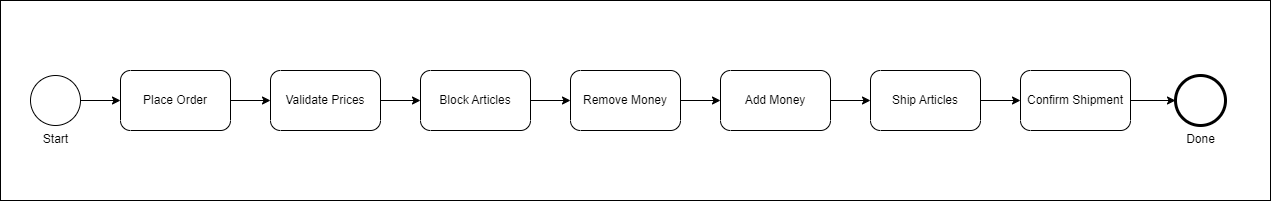
\includegraphics[width=\linewidth]{figures/SimplifiedBusinessProcess.png}
	\caption{Vereinfachte Darstellung eines Bestell- und Lieferprozesses}
\end{figure}


% TODO Diagramm für den vereinfachten Prozess

Die zum Prozess gehörenden Schritte sind folgende:

\subparagraph*{Entgegennehmen der Bestellung} Die Bestellung wird über ein imaginäres Frontend entgegengenommen. Dieses Frontend baut einen Request auf und sendet diesen per Http-Schnittstelle an das Backend. Dort wird der Request entgegengenommen und muss alle für die Abwicklung der Bestellung erforderlichen Daten enthalten. Dazu gehören der bestellende Nutzer, die geforderten Artikel und die Zahlungsinformationen. Beim Entgegennehmen wird die Bestellung initialisiert.

\subparagraph*{Validierung des Preises} Der Bestellungsrequest enthält eine Liste von den gewünschten Produkten und dem bekannten Preis pro Produkt. Um zu überprüfen, ob der dem Nutzer (dem Frontend) bekannte Preis mit dem aktuellen Preis übereinstimmt, muss dieser validiert werden. % TODO warum ist dieser Schritt notwendig	

\subparagraph*{Blockieren der Artikel} Die geforderten Artikel sollten für diese Bestellung reserviert werden, bis der Bestellvorgang abgeschlossen ist. In einem Online-Shop wird angezeigt, wieviele Artikel auf Lager vorrätig sind. Beim Blockieren der Artikel wird dieser Betrag verändert. Somit sehen andere Nutzer nach Ausführung dieses Schrittes den aktuellen Wert der vorrätigen Artikel. 

\subparagraph*{Zahlungsabwicklung} Der berechnete Preis der Bestellung muss vom Konto des Kunden abgebucht werden. Das Konto des Händlers erhält denselben Betrag gutgeschrieben. Die Konten des Kunden und des Online-Shop-Besitzers müssen nicht bei derselben Bank liegen. 

\subparagraph*{Auslösen der Lieferung} Die blockierten Artikel werden versendet. Dieser Prozess dauert einen längeren Zeitraum an.

\subparagraph*{Abschluss der Lieferung} Der Lieferant bestätigt die Übergabe der Waren an den Kunden.


\paragraph*{Implementierung}

Nachdem der Geschäftsprozess definiert wurde, soll das Saga-System implementiert werden. In \ref{sec_saga_formalisierung_dea} wurde erläutert, wie die im Koordinator laufende SEC beschrieben werden kann. Die Implementierung soll durch diese Darstellungsform beschrieben werden können.

Für die Transaktionsteilnehmer gilt zu Beginn der Implementierung lediglich die Anforderung, dass die Schnittstellen per Request-Response-Muster aufgerufen werden. Dafür wird das Http-Protokoll verwendet.

